\documentclass{standalone}
\usepackage{tikz}
\usetikzlibrary{arrows,decorations.markings,calc,positioning}

% "Add arrows to a smooth tikz function"
% from http://tex.stackexchange.com/a/163695
\tikzset{
   set arrow inside/.code={\pgfqkeys{/tikz/arrow inside}{#1}},
   set arrow inside={end/.initial=>, opt/.initial=},
   /pgf/decoration/Mark/.style={
      mark/.expanded=at position #1 with
      {
         \noexpand\arrow[\pgfkeysvalueof{/tikz/arrow inside/opt}]{\pgfkeysvalueof{/tikz/arrow inside/end}}
      }
   },
   arrow inside/.style 2 args={
      set arrow inside={#1},
      postaction={
         decorate,decoration={
            markings,Mark/.list={#2}
         }
      }
   },
}

\begin{document}%
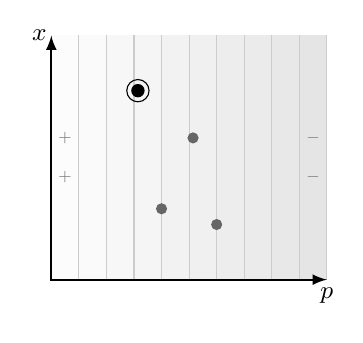
\begin{tikzpicture}[font=\small]

\clip (-0.3,-0.45) rectangle (3.6,3.2);

% contours
\begin{scope}
   \clip (0,0) rectangle (3.5,3.1);
   \foreach \s in {10,...,1}
   {
      \begin{scope}[shift={($(0.35*\s,0.35*\s)$)}]
      
         \draw[black!20,fill=black!\s]
            (-5.0,5.0) rectangle (0.0,-5.0);
         
      \end{scope}
   }
\end{scope}

\node[text=black!50] at (0.175,1.3) {\tiny $+$};
\node[text=black!50] at (0.175,1.8) {\tiny $+$};
\node[text=black!50] at (3.325,1.3) {\tiny $-$};
\node[text=black!50] at (3.325,1.8) {\tiny $-$};

%\draw[black!5] (-0.1,-0.1) rectangle (3.6,3.6);

%\draw[black!50] (-0.1,0.7) -- (3.5,0.7); % optimal path
%\node at (1.75,0.9) {\scriptsize Optimal Path};

% simple point
%\node[circle,fill=black,inner sep=0.07cm] at (1.5,3) {};
%\node[circle,fill=black,inner sep=0.05cm] (a1) at (1.0,2.7) {};
%\node[above right=-0.1cm of a1] {$A_1$};

\node[circle,fill=black,inner sep=0.06cm] at (1.1,2.4) {};
\node[circle,draw=black,inner sep=0.1cm] at (1.1,2.4) {};
\node[circle,fill=black!60,inner sep=0.05cm] at (1.4,0.9) {};
\node[circle,fill=black!60,inner sep=0.05cm] at (1.8,1.8) {};
\node[circle,fill=black!60,inner sep=0.05cm] at (2.1,0.7) {};
%\node[above right=-0.1cm of a2] {$A_2$};

% anytime
%\draw[black,thick,->,
%   arrow inside={end=>,opt={black}}{0.25,0.5,0.75}]
%   (0.84,2.45)
%   .. controls (1.05,1.96) and (1.54,1.96) .. (1.96,1.75)
%   .. controls (2.38,1.54) and (2.67,0.84) .. (3.50,0.77);
%\node[circle,fill=black,inner sep=0.07cm] at (2.45,1.33) {};

% axes
\draw[thick,latex-latex] (3.5,0) -- (0,0) -- (0,3.1);

% labels
\node at (3.5,-0.2) {$p$};
\node at (-0.15,3.1) {$x$};

%\node at (-0.2,0.75) {$x^*$};

%\node[anchor=east,inner sep=0pt] at (3.5,0.2) {\scriptsize Planning Effort $\rightarrow$};
%\node[rotate=90,anchor=east,inner sep=0pt] at (0.2,3.5) {\scriptsize Execution Effort $\rightarrow$};

\end{tikzpicture}%
\end{document}
